\documentclass[tikz,border=6pt]{standalone}
\usepackage{fontspec}
\usepackage{xeCJK}
\setmainfont{Times New Roman}
\setCJKmainfont{Hiragino Sans GB}
\setCJKsansfont{Microsoft YaHei}
\setCJKmonofont{STSong}
\usepackage{xcolor}
\usetikzlibrary{arrows.meta}

\definecolor{wiregray}{HTML}{333333}
\definecolor{nodeorange}{HTML}{F0AD4E}
\definecolor{blockblue}{HTML}{4A90D9}

\begin{document}
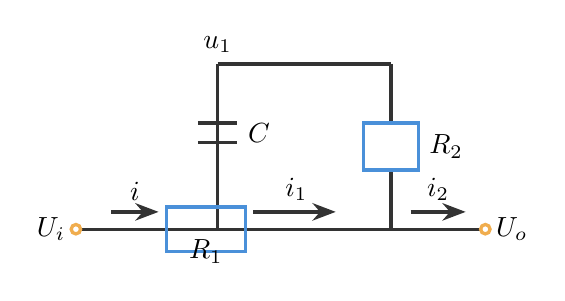
\begin{tikzpicture}[line width=1.2pt, >=Stealth]
  \draw[wiregray] (0,0) -- (1,0);
  \draw[wiregray] (1,0) -- (2.6,0);
  \draw[wiregray] (2.6,0) -- (5.2,0);
  \draw[wiregray] (1.8,0) -- (1.8,2.1);
  \draw[wiregray] (1.55,1.1) -- (2.05,1.1);
  \draw[wiregray] (1.55,1.35) -- (2.05,1.35);
  \draw[wiregray] (1.8,2.1) -- (4.0,2.1);
  \draw[wiregray] (4.0,2.1) -- (4.0,1.35);
  \draw[wiregray] (4.0,0.75) -- (4.0,0);

  \draw[blockblue] (1.15,-0.28) rectangle (2.15,0.28);
  \draw[blockblue] (3.65,0.75) rectangle (4.35,1.35);

  \filldraw[fill=white, draw=nodeorange] (0,0) circle (1.7pt);
  \filldraw[fill=white, draw=nodeorange] (5.2,0) circle (1.7pt);

  \node[left] at (0,0) {$U_i$};
  \node[right] at (5.2,0) {$U_o$};
  \node[above] at (1.8,2.1) {$u_1$};
  \node[below] at (1.65,0) {$R_1$};
  \node[right] at (4.35,1.05) {$R_2$};
  \node[right] at (2.05,1.22) {$C$};

  \draw[wiregray, ->] (0.45,0.22) -- (1.05,0.22);
  \node[above] at (0.75,0.22) {$i$};
  \draw[wiregray, ->] (2.25,0.22) -- (3.3,0.22);
  \node[above] at (2.8,0.22) {$i_1$};
  \draw[wiregray, ->] (4.25,0.22) -- (4.95,0.22);
  \node[above] at (4.6,0.22) {$i_2$};
\end{tikzpicture}
\end{document}
